\documentclass[UTF8]{ctexart}
\usepackage{graphicx}
\usepackage{amsmath}
\usepackage{amssymb}

\begin{document}

\section{作业}

\subsection{1}

考虑二维两点边值问题 \(P_{2D}\)

\[\begin{aligned}
 - \mathrm{\Delta}u = f & ,\quad\text{ in }\Omega \\
u = 0 & ,\quad\text{ on }\Gamma
\end{aligned}\]

其对应的变分问题(\(W_{2D}\)):找到 \(u \in V\),满足

\[a(u,v) = (f,v)\quad\forall v \in V\]

极小化问题(\(M_{2D}\)):找到 \(u \in V\)

\[J(u) \leq J(v)\quad\forall v \in V\]

\subsubsection{{(1) 写出 \(J\) 和 \(a\)
的表达式}{(1) 写出 J 和 a 的表达式}}

\[a(u,v) = \int_{\Omega}\nabla u \cdot \nabla vdx\]

\[J(u) = \frac{1}{2}a(u,u) - (f,u)\]

\[V = H_{0}^{1}\]

\subsubsection{(2) 证明等价性:}

\paragraph{{P \(\Rightarrow\)
W}}

因为 \[\begin{aligned}
 - \mathrm{\Delta}u = f & ,\quad\text{ in }\Omega \\
u = 0 & ,\quad\text{ on }\Gamma
\end{aligned}\] 那么:\(\forall v \in V\),因为
\(v|_{\partial\Omega} = 0\)

\[\begin{aligned}
(f,v) & = ( - \mathrm{\Delta},v) \\
 & = \int_{\Omega}\nabla u \cdot \nabla vdx - \int_{\partial\Omega}v\frac{\partial u}{\partial n}dS \\
 & = \int_{\Omega}\nabla u \cdot \nabla vdx \\
 & = a(u,v)
\end{aligned}\]

因此原问题的解 \(u\) 是变分问题的解。

\paragraph{{W \(\Rightarrow\)
M}}

\(\forall v \in V\):

\[\begin{aligned}
J(v) & = J\left( u + (v - u) \right) \\
 & = \frac{1}{2}a(u,u) + a(v - u,u) + a(v - u,v - u) - (f,v) \\
 & = \frac{1}{2}a(u,u) + (f, - u) + a(v - u,v - u) \\
 & \geq J(u)
\end{aligned}\]

因此 \(u\) 是极小化问题的解。

\paragraph{{M \(\Rightarrow\)
W}}

\(\forall v \in V\):考虑\(\varepsilon\)的函数\(f\):

\[f(\varepsilon) = J(u + \varepsilon v) = \frac{1}{2\left( a(u,u) + 2\varepsilon a(u,v) + \varepsilon^{2}a(v,v) \right)} - (f,u + \varepsilon v)\]

对 \(\varepsilon\) 求导

\[f\prime(\varepsilon) = \varepsilon a(v,v) + a(u,v) - (f,v)\]

因为 \(J(u) \leq J(v)\quad\forall v \in V\) ,那么

\[f\prime(0) = a(u,v) - f(v) = 0\]

因为上式对 \(\forall v \in V\) 成立,所以\(u\)也是变分问题的解。

\paragraph{{W \(\Rightarrow\)
P}}

因为 \(u\) 充分光滑,并利用\(v|_{\partial\Omega} = 0\),Green公式:

\[\int_{\Omega}v( - \mathrm{\Delta}u)dx = \int_{\Omega}\nabla u \cdot \nabla vdx\]

\[0 = a(u,v) - (f,v) = \int_{\Omega}( - \mathrm{\Delta}u - f)vdx\]

假设 \(\exists x_{0} \in \Omega\),使得 \(\mathrm{\Delta}u + f > 0\)
对以 \(x_{0}\) 为球心的 \(B\)恒成立,取
\(v\)为以\(B\)为支集的函数,在\(B\)内满足\(v > 0\),那么:
\[\int_{\Omega}(\mathrm{\Delta}u + f)vdx = \int_{B}(\mathrm{\Delta}u + f)vdx > 0\]

因此这样的 \(x_{0}\) 不存在,从而 \(u\) 是原方程的解。

\subsection{Brenner 0.x.9}

Let \(V\) denote the space, and \(a( \cdot , \cdot )\) the binlinear
form. Prove the following coercivity result
\[\left. \parallel v \right.\parallel^{2} + \left. \parallel{v\prime} \right.\parallel^{2} \leq Ca(v,v)\]
Give the value for \(C\). (Hint: see the hint in 0.x.6. For simplicity,
restrict the result to \(v \in V \cup C^{1}(0,1)\))

Hint in 0.x.6: 若 \(w(0) = 0,w \in L^{2}(0,1),a(w,w) < \infty\),考虑
\(w\) 的傅立叶变换:

\[w(t) = \sum_{n = 1}^{\infty}a_{n}\sin\frac{n\pi}{2}x\]

那么:

\[\int_{0}^{1}\left( w(t) \right)^{2}dx = \frac{1}{2}\sum_{n = 1}^{\infty}a_{n}^{2}\]

考虑 \(w\prime\) 的傅立叶变换:

\[w\prime(t) = \sum_{n = 1}^{\infty}a_{n}\frac{n\pi}{2}\cos\frac{n\pi}{2}x\]

那么:

\[\int_{0}^{1}\left( w\prime(t) \right)^{2}dx = \frac{1}{2}\sum_{n = 1}^{\infty}\left( a_{n}\frac{n\pi}{2} \right)^{2}\]

公式 \(\int_{0}^{1}w(t)\hat{}2dx \leq c\int_{0}^{1}w\prime(t)\hat{}2dx\)
中的 \(c\)
在:\(a_{1} = 1,a_{n} = 0\quad(n \geq 2)\)时取最大值:\(c = \frac{4}{\pi^{2}}\)

因此:\[\int_{0}^{1}w(t)\hat{}2dx \leq \frac{4}{\pi^{2}}\int_{0}^{1}w\prime(t)\hat{}2dx\]

即
\(\left. \parallel w \right.\parallel^{2} \leq \frac{4}{\pi^{2}}\left. \parallel{w\prime} \right.\parallel^{2}\)

\textbf{Proof:}
\(V = \left\{ v \in L^{2}(0,1):a(v,v) < \infty\text{ and }v(0) = 0 \right\}\),

\[a(v,v) = \int_{0}^{1}v\prime(t)\hat{}2dt = \left. \parallel{v\prime} \right.\parallel^{2}\]
那么:
\[\left. \parallel v \right.\parallel^{2} + \left. \parallel{v\prime} \right.\parallel^{2} \leq \left( 1 + \frac{4}{\pi^{2}} \right)a(v,v)\]
即 \(C = 1 + \frac{4}{\pi^{2}}\)

\subsection{Brenner 0.x.10}

Let \(V\) denote the space, and \(a( \cdot , \cdot )\) the binlinear
form. Prove the following version of sobolev's inequality:
\[{\left. \parallel v \right.\parallel^{2}}_{\max} \leq Ca(v,v)\] Give
the value for \(C\). (Hint: see the hint in 0.x.6. For simplicity,
restrict the result to \(v \in V \cup C^{1}(0,1)\))

\textbf{Proof:} 因为\(\left( \sup|v| \right)^{2} = \sup v^{2}\),利用
Cauchy不等式:

\[\begin{aligned}
v(t) & = \int_{0}^{t}v\prime(x)dx \\
 & = \int_{0}^{t}1 \cdot v\prime(x)dx \\
 & \leq \sqrt{t}\sqrt{\int_{0}^{t}v\prime(x)\hat{}2dx}
\end{aligned}\]

那么: \[v(t)\hat{}2 \leq t\int_{0}^{t}v\prime(x)\hat{}2dx\]

两边同取上确界:
\[\sup v^{2} \leq \sup\left( t\int_{0}^{t}v\prime(x)\hat{}2dx \right) \leq \int_{0}^{1}v\prime(x)\hat{}2dx\]

因此:

\[\left. \parallel v \right.\parallel_{\max}^{2} \leq a(v,v)\quad\forall v \in V\]

即题目中常数 \(C = 1\),取 \(v(x) = x\) 可使上式成立。

\subsection{Johnson 1.7}

Formulate a difference method for 1.16 in the case when \(\Omega\) is
square \[\begin{cases}
 - \mathrm{\Delta} & \begin{array}{rlr}
u & = f & \quad\text{ in }\Omega
\end{array} \\
 & \begin{array}{rlr}
u & = 0 & \quad\text{ on }\Omega
\end{array}
\end{cases}\] using the difference approximation
\[\frac{\partial^{2}u}{\partial x_{1}^{2}}\sim\frac{u\left( x_{1} + h,x_{2} \right) - 2u\left( x_{1},x_{2} \right) + u\left( x_{1} - h,x_{2} \right)}{h^{2}}\]
and a corresponding approximation for
\(\frac{\partial^{2}u}{\partial x_{2}^{2}}\). Compare with example 1.1.

在这一题,我们沿用 Example 1.1 的记号。对于非边界点\(i\),利用上述公式:

\[\frac{\partial^{2}u}{\partial x_{1}^{2}} \approx \frac{u_{i + N} + u_{i - N} - 2u_{i}}{h^{2}}\]
\[\frac{\partial^{2}u}{\partial x_{1}^{2}} \approx \frac{u_{i + 1} + u_{i - 1} - 2u_{i}}{h^{2}}\]

泊松方程改写为差分方程如下:

\[- \left( \frac{u_{i + N} + u_{i - N} - 2u_{i}}{h^{2}} + \frac{u_{i + 1} + u_{i - 1} - 2u_{i}}{h^{2}} \right) = f\left( x_{i} \right)\]

简化为:

\[- u_{i + 1} + 4u_{i} - u_{i - 1} - u_{i - N} - u_{i + N} = h^{2}f\left( x_{i} \right)\]

假设 \(f(x)\) 充分光滑,那么有限元法中,方程组右端的 \(b_{i}\)
可以近似为:
\[b_{i} = \int\varphi_{i}f(x)dx = h^{2}\left( f\left( x_{i} \right) + O(h) \right)\]

观察差分方程获得的方程组和右端项,可以发现在这种近似的情况下,两个方法获得的方程组是相同的。

\begin{figure}
\centering
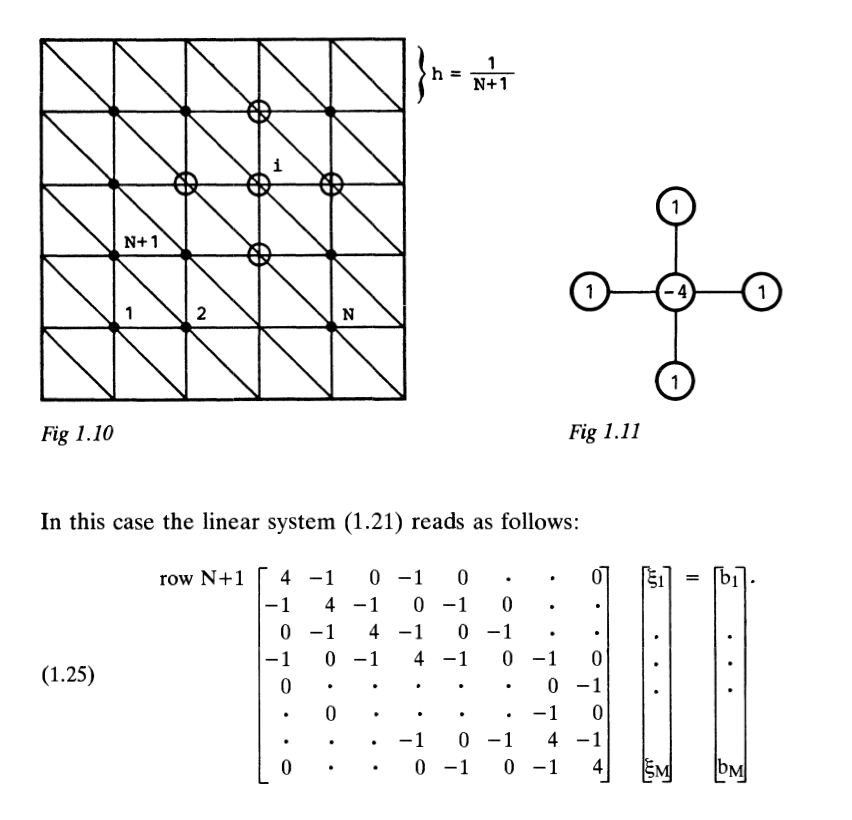
\includegraphics[width=0.7\textwidth]{jh17.png}
\caption{Example 1.1}
\end{figure}

\subsection{Johnson 1.15}

Prove that (1.35) and (1.36) are equivalent (cf the proof of theorem
1.1).

1.35: \[
{{\langle u - u_{h},v\rangle} = 0\quad\forall v \in V_{h}}{}\]

1.36: \[
{\left. \parallel{u - u_{h}} \right.\parallel_{H^{1}(\Omega)} \leq \left. \parallel{u - v} \right.\parallel_{H^{1}(\Omega)}\quad\forall v \in V_{h}}{}\]

\textbf{Proof:} 1.35 \(\Rightarrow\) 1.36:
\(\forall v \in V_{h},u_{h} - v \in V_{h}\) 那么:
\[{\langle u - u_{h},u_{h} - v\rangle} = 0\]

因此:

\[\begin{aligned}
\left. \parallel{u - v} \right.\parallel_{H^{1}}^{2} & = {\langle u - v,u - v\rangle} \\
 & = {\langle u - u_{h} + u_{h} - v,u - u_{h} + u_{h} - v\rangle} \\
 & = {\langle u - u_{h},u - u_{h}\rangle} + {\langle u - v,u - v\rangle} \\
 & \geq \left. \parallel{u - u_{h}} \right.\parallel_{H^{1}}
\end{aligned}\]

因此1.36成立。下证1.36\(\Rightarrow\)1.35,\(\forall v \in V_{h}\),定义如下的函数:

\[f(\varepsilon) = \left. \parallel{u - u_{h} + \varepsilon v} \right.\parallel_{H^{1}}\]

因为1.36成立,所以 \(f'(0) = 0\),立刻得到:

\[{\langle u - u_{h},v\rangle} = 0\]

即 1.35成立。综上1.35与1.36等价。

\subsection{Johnson 1.16}

Show that the problem

\[\begin{cases}
 - u\prime\prime = f \\
u(0) = u\prime(1) = 0
\end{cases}\]

can be given the follow variational formulation: Find \(u \in V\) such
that \[(u\prime,v\prime) = (f,v)\quad\forall v \in V\] where
\(V = \left\{ v \in H^{1}(I):v(0) = 0 \right\}\). Formulate a Finite
element method for this problem using piecewise linear functions.
Determine the corresponding linear system of equations in the case of a
uniform partition and study in particular how the boundary condition
\(u\prime(1) = 0\) is approximated by the method.

\textbf{Solution:}

首先说明变分问题和原问题是等价的。若 \(u\) 是原问题的解,那么
\(\forall v \in V\): \[\begin{aligned}
(u\prime,v\prime) & = u\prime(1)v(1) - u\prime(0)v(0) - (u\prime\prime,v) \\
 & = (f,v)
\end{aligned}\] 因此 \(u\) 是变分问题的解。另一方面若 \(u\)
是变分问题的解: \[u\prime(1)v(1) = (u\prime\prime + f,v)\] 假设
\(\exists x_{0},u\prime\prime + f > 0\),若解是光滑的,那么存在区间
\(\left\lbrack x_{1},x_{2} \right\rbrack\)
\(u\prime\prime + f > 0\quad\forall x_{1} < x < x_{2}\)

这说明,取 \[v = \begin{cases}
 - \left( x - x_{1} \right)\left( x - x_{2} \right) & \quad x_{1} < x < x_{2} \\
0 & \quad\text{ otherwise }
\end{cases}\]

有 \[0 = u\prime(1)v(1) = (u\prime\prime + f,v) > 0\]

因此 \((u\prime\prime + f,v) = 0\quad\forall v \in V\),另外,取
\(v(x) = x\),可得到 \(u\prime(1) = 0\)。所以变分问题的解是原问题的解。

下面描述其有限元解:取
\(V_{h} = \left\{ v:v\text{ 为分片连续线性函数},v(0) = 0 \right\}\)。有限元解为:找
\(u_{h} \in V_{h}\),使得
\[\left( u_{h}\prime,v_{h}\prime \right) = \left( f,v_{h} \right)\quad\forall v \in V_{h}\]

设
\(0 = x_{0} < x_{1} < \cdots < x_{n} < x_{n} = 1,\quad h = x_{i} - x_{i - 1}\)
全局基函数为 \[\varphi_{i} = \begin{cases}
\frac{x - x_{i - 1}}{x_{i} - x_{i - 1}} & \quad x_{i - 1} \leq x < x_{i} \\
\frac{x_{i + 1} - x}{x_{i + 1} - x_{i}} & \quad x_{i} \leq x < x_{i + 1} \\
0 & \quad\text{ otherwise }
\end{cases},\quad\quad\varphi_{n} = \begin{cases}
\frac{x - x_{n - 1}}{x_{n} - x_{n - 1}} & \quad x_{n - 1} < x \leq 1 \\
0 & \quad\text{ otherwise }
\end{cases}\]

那么 \[u_{h} = \sum_{i = 1}^{n}u_{h}\left( x_{i} \right)\varphi_{i}\]
计算全局刚度矩阵:

\[\left( \varphi_{i}\prime,\varphi_{i}\prime \right) = \frac{2}{h},\quad\left( \varphi_{i}\prime,\varphi_{i - 1}\prime \right) = \left( \varphi_{i - 1}\prime,\varphi_{i}\prime \right) = - \frac{1}{h}\quad\forall i < n\]

对于 \(i = n\):

\[\left( \varphi_{n}\prime,\varphi_{n}\prime \right) = \frac{1}{h},\left( \varphi_{n}\prime,\varphi_{n - 1}\prime \right) = - \frac{1}{h}\]

因此全局刚度矩阵为:

\[K = \frac{1}{h}\begin{pmatrix}
2 & - 1 & 0 & \cdots & 0 & 0 \\
 - 1 & 2 & - 1 & \cdots & 0 & 0 \\
0 & - 1 & 2 & \cdots & 0 & 0 \\
 \vdots & \vdots & \vdots & \ddots & \vdots & \vdots \\
0 & 0 & 0 & - 1 & 2 & - 1 \\
0 & 0 & 0 & 0 & - 1 & 1
\end{pmatrix}\]

\[f_{i} = \left( f,\varphi_{i} \right) \approx \frac{1}{h}f\left( x_{i} \right)\quad f_{n} = \left( f,\varphi_{n} \right) \approx \frac{1}{2h}f(1)\]

将节点值组合成向量:\(U = \left( u_{h}\left( x_{1} \right),u_{h}\left( x_{2} \right),\ldots,u_{h}\left( x_{n} \right) \right)^{T}\)那么有限元法求解如下的线性方程组:

\[KU = F\]

\subsection{1.17}

Show that the problem (M) and (V) of this section are equivalent.

(V): Find \(u \in H^{1}(\Omega)\), s.t. \[a(u,v) = (f,v) + < g,v >\]
where \(a(u,v) = \int_{\Omega}(\Delta u \cdot \Delta v + uv)dx\)

(M): Find \(u \in H^{1}\) such that
\(F(u) \leq F(v)\quad\forall v \in H^{1}(\Omega)\) where
\[F(v) = \frac{1}{2}a(v,v) - (f,v) - < g,v >\]

\textbf{Proof: } 假设 \(u\) 是 (V) 的解,\(\forall v \in V\),因为
\(u - v \in V\),那么: \[a(u,u - v) = (f,u - v) + < g,u - v >\] 那么:
\[\begin{array}{rlr}
F(v) & = F\left( u + (v - u) \right) = \frac{1}{2}a(u,u) + \frac{1}{2}a(v - u,v - u) - (f,u) - < g,u > \\
 & = F(u) + \frac{1}{2}a(v - u,v - u) & \geq F(u)
\end{array}\] 因此 \(u\) 是 (M) 的解。

假设 \(u\) 是 (M) 的解,定义如下的函数
\[f(\varepsilon) = F(u + \varepsilon v)\] 因为
\(F(u) \leq F(v)\ \forall v \in V\),所以\(\varepsilon = 0\)是 \(f\)
的极小点,即有 \(f\prime(\varepsilon) = 0\),化简得到:
\[a(u,v) - (f,v) - < g,v > = 0\] 因此 \(u\) 是 (V) 的解。

\subsection{1.18}

Let \(\Omega\) be a bounded domain in the plane and let the boundary
\(\Gamma\) of \(\Omega\) be devided into two parts \(\Gamma_{1}\) and
\(\Gamma_{2}\). Give a variational formulation of the following problem:
\[\begin{cases}
\mathrm{\Delta}u = f & \quad\text{ in }\Omega \\
u = u_{0} & \quad\text{ on }\Gamma_{1} \\
\frac{\partial u}{\partial n} = g & \quad\text{ on }\Gamma_{2}
\end{cases}\] where \(f,u_{0}\) and \(g\) are given functions. Then
formulate a finite element method for this problem. Also give an
interpretation of this problem in mechanics or physics.

\textbf{Solution: }

Varitional Formulation: Find \(u \in {\mathbb{V}}\), such that:
\[a(u,v) = (f,v) + < g,v > \forall v \in {\mathbb{V}}_{0}\] where
\[{\mathbb{V}} = \left\{ v \in H^{1}:v|_{\Gamma_{1}} = u_{0} \right\},\quad{\mathbb{V}}_{0} = \left\{ v \in H^{1}:v|_{\Gamma_{1}} = 0 \right\}\]
\[a(u,v) = \int_{\Omega}\nabla u \cdot \nabla vdx\]
\[(f,v) = \int_{\Omega}fvdx\] \[< g,v > = \int_{\Gamma_{2}}gvdS\] then
\(\forall v \in {\mathbb{V}}_{0}\): \[\begin{aligned}
\int_{\Omega}( - \mathrm{\Delta}u)vdx & = \int_{\Omega}\nabla u \cdot \nabla vdx - \int_{\Gamma_{2}}v\frac{\partial u}{\partial n}dS
\end{aligned}\]

设\(u\)为原问题的解:
\[\int_{\Omega}fvdx = \int_{\Omega}( - \mathrm{\Delta}u)vdx\]
利用上式,有:
\[\int_{\Omega}\nabla u \cdot \nabla vdx = \int_{\Omega}fvdx + \int_{\Gamma_{2}}gvdS\]
因此原问题的解是变分问题的解。

设 \(u\) 是变分问题的解:
\[\int_{\Omega}( - \mathrm{\Delta}u)vdx = \int_{\Omega}fvdx + \int_{\Gamma_{2}}gvdS - \int v\frac{\partial u}{\partial n}dS\]
整理得:
\[\int_{\Omega}(\mathrm{\Delta}u + f)vdx = \int_{\Gamma_{2}}v\left( g - \frac{\partial u}{\partial n} \right)dS\]

\[\int_{\Omega}(\mathrm{\Delta}u + f)vdx = \int_{\Gamma_{2}}vgdS\]

如果\(u\prime\prime + f\)充分光滑,且在 \(x_{0} \in \Omega\)
\(\mathrm{\Delta}u + f > 0\),那么存在 \(v \in {\mathbb{V}}_{0}\) 在
\(v|_{\partial\Omega} = 0\) 使得
\[0 = \int_{\Omega}(\mathrm{\Delta}u + f)vdx > 0\] 因此
\(u\prime\prime + f = 0\ \forall x \in \Omega\),且
\(\int_{\Omega}(\mathrm{\Delta}u + f)vdx = 0\)。 这说明
\(\int_{\Gamma_{2}}v\left( g - \frac{\partial u}{\partial n} \right)dS = 0\ \forall v \in {\mathbb{V}}_{0}\),同理可得
\(g - \frac{\partial u}{\partial n} = 0\)。

因此\(u\)也是原问题的解。这说明我们构造的变分问题和原问题的解是等价的。

FEM的构造如下。考虑
\({\mathbb{V}}_{h} ≔ \left\{ v:v\text{ 为分片线性函数},v|_{\Gamma_{1}} = u_{0} \right\},{\mathbb{V}}_{h0} = \left\{ v:v\text{ 为分片线性函数},v|_{\Gamma_{1}} = 0 \right\}\),找
\(u \in {\mathbb{V}}_{h},\) s.t.
\[a(u,v) = (f,v) + < g,v > \quad\forall v \in {\mathbb{V}}_{h0}\]

物理解释为:设有线性弹性模型控制的材料,其构型空间为
\(\Omega\),定义\(\Omega\)上的形变为将\(x \in \Omega\)形变到\(n\)维空间的\(u(x)\)。因为材料为线性材料,假设在构型空间的每一点有外力,那么其稳定状态的控制方程可以写为:
\[- \mathrm{\Delta}_{x}u(x) = f\] 对于材料边界
\(\partial\Omega\),一部分\(\Gamma_{1}\)是固定边界,即有
\[u = u_{0}\quad\text{ on }\Gamma_{1}\]
另一部分为受给定负载(外力)的边界 \(\Gamma_{2}\),那么:
\[\frac{\partial u}{\partial n} = g\quad\text{ on }\Gamma_{2}\]
即得到原本的定解问题。
\end{document}